
\begin{frame}
  \frametitle{Training Set Database: Labels}
    \begin{table}
      \footnotesize
      \centering
      \begin{tabular}{@{}lll@{}}
      \toprule
        \textbf{PWR} & \textbf{BWR}  & \textbf{PHWR} \\ \toprule
        CE14x14      & GE7x7-0       & CANDU19       \\
        W17x17       & Abb8x8-1      & CANDU28       \\
        S18x18       & Atrium10x10-9 & CANDU37       \\
        BW15x15      & SVEA64-1      &               \\
        VVER440      &               &               \\
        VVER1000     &               &               \\ \bottomrule
      \end{tabular}
      \caption{ORIGEN designations for reactor technologies and fuel assemblies.}
    \end{table}
  \vspace{-8pt}
    \begin{table}
      \footnotesize
      \centering
      \begin{tabular}{@{}llll@{}}
        \toprule
        & \textbf{PWR}              & \textbf{BWR}              & \textbf{PHWR} \\  \toprule
        Power Density [$MW/MTU$]                        
        & 25, 35, 41                & 10, 22                    & 2.2, 18, 22   \\
        \boxalert{Burnup} [$GWd/MTU$]                   
        & 2--68                     & 1--68                     & 0.45--12.6    \\
        Moderator Density [$g/cm^3$]                    
        & 0.71                      & \{0.1, 0.3, 0.5, 0.7\}    & 0.84          \\
        \boxalert{Enrichment} [$\%\:{}^{235}{\text{U}}$]
        & \{0.5, 1.5, 2, 3, 4, 5\}  & \{0.5, 1.5, 2, 3, 4, 5\}  & 0.711         \\
        \boxalert{Cooling Time} [$days$]                
        & \multicolumn{3}{c}{\{0--6000\} in 100-day steps}                      \\ \bottomrule
      \end{tabular}
      \caption{Simulation parameters for ORIGEN input files.}
    \end{table}
\end{frame}


\begin{frame}
  \frametitle{Training Set Database: Labels}
  \begin{figure}
    \centering
      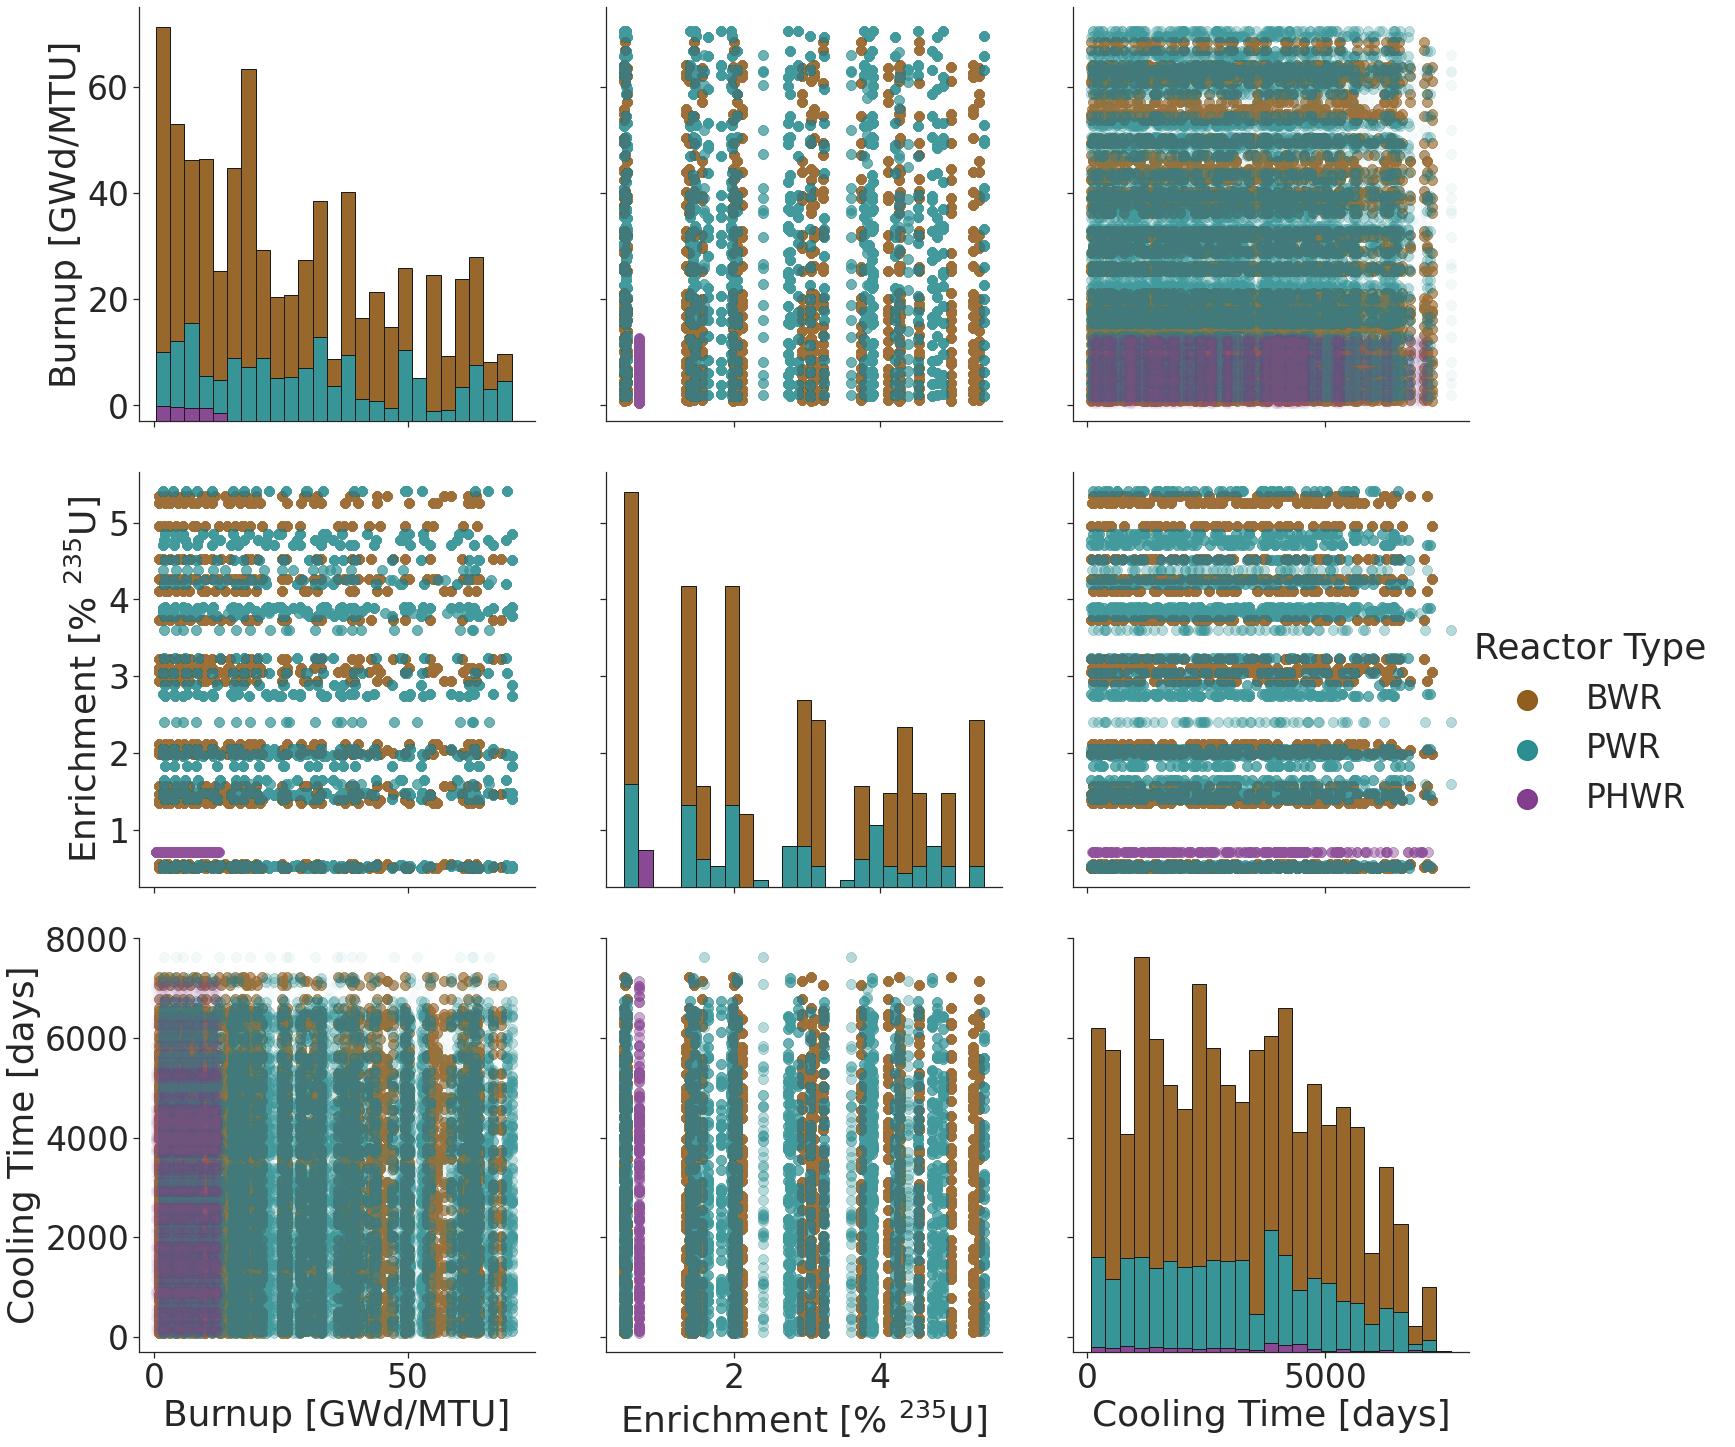
\includegraphics[height=0.8\textheight]{./figures/histogram_scatter_trainset_viz.png}
      \caption{Visualization of the training set labels (same for all scenarios).}
  \end{figure}
\end{frame}

\begin{frame}
  \frametitle{Training Set Database: Features}
    \begin{table}
      %\small
      \centering
      \renewcommand{\arraystretch}{1.3}
      \begin{tabular}{@{}|l|l|l|l|l|l|l|l|@{}}
        \hline
        \allbold{${}^{241}\text{Am}$} & ${}^{242m}\text{Am}$ &
        \allbold{${}^{243}\text{Am}$} & ${}^{242}\text{Cm}$ &
        \allbold{${}^{244}\text{Cm}$} & \allbold{${}^{134}\text{Cs}$} &
        \allbold{${}^{137}\text{Cs}$} & \allbold{${}^{154}\text{Eu}$} \\  
        \hline
        ${}^{143}\text{Nd}$ & ${}^{144}\text{Nd}$ & ${}^{145}\text{Nd}$ &
        ${}^{146}\text{Nd}$ & ${}^{148}\text{Nd}$ & ${}^{150}\text{Nd}$ &
        \allbold{${}^{237}\text{Np}$} & \allbold{${}^{238}\text{Pu}$} \\ 
        \hline
        \allbold{${}^{239}\text{Pu}$} & \allbold{${}^{240}\text{Pu}$} &
        ${}^{241}\text{Pu}$ & ${}^{242}\text{Pu}$ & ${}^{147}\text{Sm}$ &
        ${}^{149}\text{Sm}$ & ${}^{150}\text{Sm}$ & ${}^{151}\text{Sm}$ \\ 
        \hline
        ${}^{152}\text{Sm}$ & \allbold{${}^{234}\text{U}$} &
        \allbold{${}^{235}\text{U}$} & ${}^{236}\text{U}$ & ${}^{238}\text{U}$ &  &
        & \\  
        \hline
      \end{tabular}
      \caption{The masses of these nuclides were saved from the ORIGEN simulations}
    \end{table}
    \vspace{-8pt}
    \begin{table}
      %\small
      \centering
      \renewcommand{\arraystretch}{1.3}
      \begin{tabular}{@{}|l|l|l|l|l|l|l|l|@{}}
        \hline
        ${}^{227}\text{Ac}$ & \allbold{${}^{241}\text{Am}$} &
        \allbold{${}^{243}\text{Am}$} & ${}^{133}\text{Ba}$ & ${}^{249}\text{Cf}$ &
        ${}^{252}\text{Cf}$ & ${}^{243}\text{Cm}$ & \allbold{${}^{244}\text{Cm}$} \\ 
        \hline
        ${}^{245}\text{Cm}$ & \allbold{${}^{134}\text{Cs}$} &
        \allbold{${}^{137}\text{Cs}$} & ${}^{152}\text{Eu}$ &
        \allbold{${}^{154}\text{Eu}$} & ${}^{166m}\text{Ho}$ & ${}^{85}\text{Kr}$ &
        ${}^{94}\text{Nb}$ \\ 
        \hline
        ${}^{236}\text{Np}$ & \allbold{${}^{237}\text{Np}$} & ${}^{231}\text{Pa}$ &
        ${}^{146}\text{Pm}$ & ${}^{236}\text{Pu}$ & \allbold{${}^{238}\text{Pu}$} &
        \allbold{${}^{239}\text{Pu}$} & \allbold{${}^{240}\text{Pu}$} \\ 
        \hline
        ${}^{226}\text{Ra}$ & ${}^{125}\text{Sb}$ & ${}^{228}\text{Th}$ &
        ${}^{229}\text{Th}$ & ${}^{232}\text{U}$  & ${}^{233}\text{U}$ &
        \allbold{${}^{234}\text{U}$}  & \allbold{${}^{235}\text{U}$}  \\ 
        \hline
      \end{tabular}
      \caption{The activities of these nuclides were saved from the ORIGEN simulations}
    \end{table}
\end{frame}

\begin{frame}
  \frametitle{Information Reduction}
  \textbf{\large Random \& Uniform Error} \\
  \bigskip
  \textit{Machine Learning Algorithms} \\ \medskip
  Introduced $0\% < E_{max} < 20\%$ random error\\ \smallskip
  Each nuclide measurement is altered by a random percentage in the range: 
  $[100-E_{max},100+E_{max}]$ for $E_{max} = \:$ 
  0, 1, 2, 5, 8, 10, 12, 15, 18, 20 \% \\
  \bigskip
  \textit{Maximum Likelihood Calculations} \\ \medskip
  Introduced uniform simulation uncertainty\\ \smallskip
  Each nuclide measurement is given a standard deviation of $1\%$, $5\%$, 
  $10\%$, $15\%$, and $20\%$ via \cite{mll_sensitivity}:
  \[
    \sigma_{Log L}^2 = \sum_i \left( 
                              \frac{x_{i,test} - x_{i,train}}{\sigma_{i,train}^2}
                              \right)^2 
                              (\sigma_{i,train}^2 + \sigma_{i,test}^2)
  \]
\end{frame}

\begin{frame}
  \frametitle{Information Reduction}
  \textbf{\large Detector Response \& Systematic Error} \\
  \medskip
  \begin{enumerate}
    \item Reduced radionuclide observation using nuclide activities to obtain gamma spectra
    \item Choose energy windows / window size
    \item Counting error ($\sqrt{n}$) injected using methods on previous slide
    \item Decrease detector energy resolution
  \end{enumerate}
  \begin{figure}[h!]
    \centering
    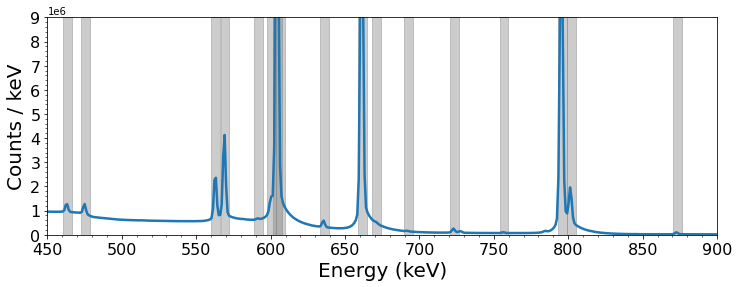
\includegraphics[height=0.4\textheight]{./figures/energy_window_example.png}
    \caption{Illustration of step 2 of the process outlined above}
  \end{figure}
\end{frame}
